\section{Lecture 15 — Applications of the Sylow Theorems}

The Sylow Theorems have two main applications/goals:
\begin{enumerate}[label=\textbf{\sffamily\color{main}(\arabic*)}]
	\item For some $n$, classify all groups with $|G|=n$.
	\item For some $n$, we can show that all groups with $|G|=n$ are not simple. Equivalently, $G$ must have a nontrivial subgroup.
\end{enumerate}

\begin{example}
	For application (1), as seen last lecture, if $|G|=pq$ with $p$ and $q$ prime, $p<q$ and $q\not\equiv 1\pmod p$. Then $G\cong\mathbb Z_{pq}$. So if $|G|=15=3\cdot 5$, then $G\cong\mathbb Z_{15}$.
\end{example}

Let's look at some examples of application (2). We rely on a variant of Corollary \ref{cor:normal_sylow_p_group}.
\begin{theorem}
	Suppose $p$ divides $|G|$. Then $G$ has a unique Sylow $p$-subgroup $P$ if and only if $P$ is normal in $G$.
\end{theorem}

\begin{example}
	Show that any group $G$ with $|G|=20=2^2\cdot 5$ is not simple.
	\begin{proof}
		By the Third Sylow Theorem (\ref{thm:sylow_3}), if $n_5$ is the number of Sylow 5-subgroups of $G$, we must have
		$$n_5\in\{1,2,4,5,10,20\},$$
		and $n_5\equiv 1\pmod 5$. The only integer satisfying this condition in the above set is 1. So $n_5=1$. Thus there is only one Sylow 5-subgroup and it must be normal. So $G$ is \underline{not} simple.
	\end{proof}
\end{example}

\begin{example}
	Show that any group $G$ with $|G|=56=2^3\cdot 7$ is not simple.
	\begin{proof}
		By the Third Sylow Theorem (\ref{thm:sylow_3}), if $n_7$ is the number of Sylow 7-subgroups of $G$, we must have
		$$\{1,8,15,22,29,36,43,50\}\quad (n_7\equiv 1\pmod 7),$$
		and
		$$n_7\in\{1,2,4,7,8,14,28,56\}\quad (n_7\text{ divides }|G|).$$
		As such, $n_7=1$ or $n_7=8$. In the case that $n_7=1$, $G$ has a unique Sylow 7-group, which must be normal and so $G$ is not simple.

		What happens if $n_7=8$? Let $P_1,P_2,\hdots, P_8$ be these 8 Sylow 7-subgroups of $G$. Note that $|P_i|=7$ for each $i$. Now for $i\neq j$, $|P_i\cap P_j|$ divides $|P_i|$ and so must be 1 or 7. But it cannot be 7 since this would imply that $P_i\cap P_j=P_i$ or $P_i\cap P_j=P_j$. So we must have that $|P_i\cap P_j|=1$.

		In total, these Sylow 7-subgroups cover $6\cdot 8+1=49$ elements of $G$. Now by the First Sylow Theorem (\ref{thm:sylow_1}), there exists a Sylow 2-group $Q$ with $|Q|=8$. Also, $|Q\cap P_i|=1$ for each $i$. So $Q$ contains $e$ and 7 other elements. Thus, $Q$ must be the unique Sylow 2-subgroup of $G$, which must be normal.

		\begin{center}
		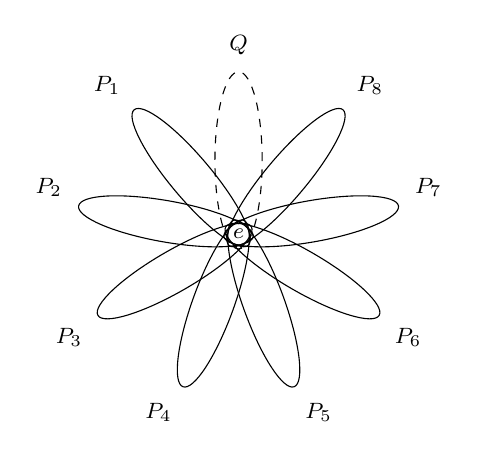
\begin{tikzpicture}[scale=0.75]
			\footnotesize
			\node (O) at (0,0) {$e$};
			\draw[dashed] (0,1.25) ellipse (0.4 and 1.5);
			\node[label=above:$Q$] at (0,2.75) {};

			\foreach \i in {1,2,...,8}{
			\draw[rotate around={{40*\i}:(O)}] (0,1.25) ellipse (0.35 and 1.5);
			\node[rotate around={{40*\i}:(O)},label=above:$P_\i$] at (0,2.75) {};
			}
		\end{tikzpicture}
		\end{center}
	\end{proof}
\end{example}

\begin{example}
	Suppose $|G|=p^nk$ with $p$ prime and $p>k$. Prove that $G$ is not simple.

	\begin{proof}
		Since $|G|=p^nk$, $G$ has at least one Sylow $p$-subgroup of order $p^n$. If $n_p$ is the number of Sylow $p$-subgroups of $G$, then $n_p\equiv 1\pmod p$. So $n_p=1+ap$, $a\in\mathbb Z$, $a\geq 0$. But also, $n_p$ divides $|G|=p^nk$. That is, $1+ap$ divides $p^nk$. But $\gcd(1+ap,p^n)=1$. So we must have $1+ap$ divides $k$. Thus, $k\geq 1+ap$. If $a\geq 1$, this means $k\geq 1+ap\geq 1+p>k$, a contradiction. So $a=0$ and thus $n_p=1$. It follows that $G$ is not simple.
	\end{proof}
\end{example}

\begin{example}
	Any group of order 33 is not simple since $33=11\cdot 3$.
\end{example}

\begin{theorem}\label{thm:commutator}
	Let $G'=\langle aba^{-1}b^{-1}\mid a,b\in G\rangle$. Then,
	\begin{enumerate}
		\item $G'$ is normal in $G$,
		\item $G/G'$ is abelian, and
		\item if $N$ is normal in $G$ and $G/N$ is abelian, then $G'\subseteq N$.
	\end{enumerate}
\end{theorem}

$G'$ as defined above is called the \textbf{commutator} of $G$.

\begin{example}
	Show all groups $G$ with $|G|=255=3\cdot 5\cdot 17$ are cyclic.

	\begin{proof}
		Since $(3\cdot 5)<17$, the previous result implies $G$ has one Sylow 17-subgroup, which is normal. Let $H$ be this Sylow 17-subgroup. Then $G/H$ is a group with order $255/17=15$. By the previous fact, $G/H\cong\mathbb Z_{15}$, which is abelian. Let $G'$ be the commutator subgroup. By Theorem \ref{thm:commutator}, $G'\subseteq H$. So $|G'|=1$ or $|G'|=17$. If $|G'|=1$, then $G/G'\cong G$ is abelian. So $G\cong\mathbb Z_3\times\mathbb Z_5\times\mathbb Z_7\cong\mathbb Z_{255}$ by the FToFAG. Now suppose $|G'|=17$. We count the number of Sylow 3-subgroups and Sylow 5-subgroups.

		\begin{center}
		\begin{tabular}{c c c}
			Divisors of 255 & mod 3 & mod 5\\ \hline
			1 & 1 & 1\\
			3 & 0 & 3\\
			5 & 2 & 0\\
			17 & 2 & 2\\
			$3\cdot 5=15$ & 0 & 0\\
			$3\cdot 17=51$ & 0 & 1\\
			$5\cdot 17=85$ & 1 & 0\\
			$3\cdot 5\cdot 17=255$ & 0 & 0
		\end{tabular}
		\end{center}

		So the number of Sylow 3-subgroups is 1 or 85 and the number of Sylow 5-subgroups is 1 or 51.

		We cannot have both 85 Sylow 3-subgroups and 51 Sylow 5-subgroups. Indeed, if $Q$ is a Sylow 3-subgroup and $P$ is a Sylow 5-subgroup, then $|Q\cap P|=1$. The Sylow 3-subgroup of order 85 consists of $2\times 85+1=170+1$ elements and the Sylow 5-subgroup of order 51 consists of $4\times 51+1=204+1$ elements, which would yield $374+1$ distinct elements, more than $|G|$.

		If there is only one Sylow 3-subgroup $Q$, then $Q$ is normal and $|G/Q|=5\cdot 17$. But then, by a theorem, this implies $G/Q\cong\mathbb Z_{5\cdot 17}$. So by Theorem \ref{thm:commutator} $G'\subseteq Q$. In particular, $|G'|=17$ and $|Q|=3$, yielding a contradiction.

		If there is only one Sylow 5-subgroup $P$, then $P$ is normal and $|G/P|=3\cdot 17$. By the same theorem, $G/P\cong\mathbb Z_{3\cdot 17}$, so $G'\subseteq P$ which would imply $|G'|=17$ divides $|P|=5$, yielding another contradiction.

		As such we must have $|G'|=1$ and so $G/G'\cong G$ is abelian.
	\end{proof}
\end{example}